\chapter{Data samples}
\section{Experimental data}
This analysis uses a sample of pp collisions collected in 2016 with the CMS 
experiment at the LHC at $\sqrt{s} = 13~\rm{TeV}$. Five primary datasets  
are used to ensure a very high trigger efficiency: MuEG, DoubleMuon, 
DoubleElectron, SingleMuon, and SingleElectron.
Only the luminosity sections are used in which all detector subsystems reported accurately.
The so-called "good run list" is furnished by the data certification working group.

%All data are analyzed using the
%\\
%\centerline{\small Cert\_271036-284044\_13TeV\_23Sep2016ReReco\_Collisions16\_JSON.txt}
%\\
%file in order to select the good luminosity sections. 

The total integrated luminosity with the associated uncertainty is $\usedLumiWithSyst$.

\subsection{Silicon strip hit efficiency loss}
\label{ss:hips}
During 2015, a reduced silicon strip hit efficiency and a reduced tracking efficiency were observed.
It was found to be correlated with the increase of the LHC instantaneous luminosity.
This is due to the effect of highly ionizing particles (HIPs) which were studied in test beams
before the tracker construction. A HIP saturates the readout chips, or APVs, of several of the strips from the hit cluster. 
The baseline is shifted toward negative values.
The chips are fully blinded in the next few bunch crossings, and remain partially blind for some time after, until they fully recover.

In total, as the instantaneous luminosity continued to increase, we observed a lower cluster charge, lower signal-to-noise ratio, lower hit efficiency, shorter tracks, and lower track efficiency.
The tracker modules most affected were wider and of higher occupancy. %mainly TOB L1 and L2. 
Any particles identified using tracks were affected by the so-called ``HIP effect.''
In particular, the electrons and muons are reconstructed from tracks and they are a crucial part of this work.

The data taken in 2016 suffered from the HIP effect until a task force was
convened to mitigate the decline in tracking performance.
The solution was found in the electronics parameters of the silicon strip readout chips.
In particular, the preamplifier feedback voltage bias (VFP) affects the duration
of the signal at the output of the preamplifier.
Reducing the VFP from 0.3 Volts to 0 Volts was found to mitigate the HIP effect. 

These 2016 data were subdivided into Run Eras labeled alphabetically.
The Run Eras used in this work are B through H. 

The HIP mitigation fix was deployed close to the demarcation of Run Eras F and G,
in the data run numbered 278803.
Run Era F comprised runs numbered (277772, 278808) and Run Era G comprised runs numbered (278820, 280385).
Due to the era-dependent nature of the HIP effect, which had a significant effect on the lepton identification, 
separate empirical corrections for leptons were derived.
They are discussed later in Chapter~\ref{chap:efficiency}.
For brevity, the corrections intended to represent the data before the fix are denoted as
``B-F'' or ``BCDEF'', despite the fact that the mitigation did not occur precisely at the Run Era changeover.
Similarly, the corrections representing the data after the fix are denoted as ``G-H'' or ``GH''.

\section{Simulated samples}
\label{sec:mcsamples}
Several Monte Carlo (MC) event generators are used to simulate the signal and
background processes. For all processes, the detector response is simulated using a detailed
description of the CMS detector, based on the \textsc{GEANT4} 
package~\cite{Agostinelli:2002hh}, and event reconstruction is performed with
the same algorithms as used for data.
The simulated samples include additional interactions per bunch crossing (pileup).
The simulated events are weighted so that the pileup distribution matches the data,
with an average pileup of about 25 interactions per bunch crossing.

\subsection{Standard Model processes}
Resonant Z boson background processes ($\W\Z$, $\Z\Z$, tribosons, etc.) are
estimated using Monte Carlo (MC) samples. Nonresonant background processes
($\ttbar$, $\tw$, $\W\W$, $\dytt$, etc.) are estimated using $\Pe\mu$ data events.

The $\W\Z$ and $\Z\Z$ processes, via $\Pq\Paq$ annihilation, 
are generated at next-to-leading-order (NLO) with 
\textsc{POWHEG2.0}~\cite{Alioli:2008gx,Nason:2004rx,Frixione:2007vw,powheg:2010}. 
The $\Pg\Pg \to \Z\Z$ process is simulated with MCFM~\cite{MCFM}. 
The $\Z\gamma$, $\ttbar \Z$, $\W\W\Z$, $\W\Z\Z$, and $\Z\Z\Z$ 
processes are generated with \textsc{MadGraph5\_aMC@NLO}~\cite{Alwall:2014hca}.
The signal samples are simulated using \textsc{MadGraph5\_aMC@NLO} at next-to-leading-order (NLO), 
\textsc{MadGraph5} at leading-order (LO), and \textsc{POWHEG} at NLO. The 
default MC generator is \textsc{MadGraph5\_aMC@NLO}. 
The \textsc{PYTHIA8}~\cite{Sjostrand:2006za,Sjostrand:2015} package is used 
for parton showering, hadronization, and the underlying event simulation,
with tune CUETP8M1.
The NNPDF 3.0~\cite{nnpdf} set is used as the default set of parton distribution 
functions (PDFs). 
The processed dataset names and cross sections for the Standard Model processes considered 
in the analysis are shown in Table~\ref{tab:mcprocess}.
Simulated datasets from the RunIISummer16MiniAODv2 campaign are used.
\clearpage
\begin{sidewaystable}[hbtp]
  \caption{Processed dataset names and cross sections for the Standard Model processes considered in the analysis.
           The processes are grouped in the following way: Resonant Diboson, Triboson, Nonresonant, and Drell-Yan.\label{tab:mcprocess}}
    \begin{center}
    {\scriptsize
      \begin{tabular}{|p{3.0cm}|p{13cm}|p{3.5cm}|}
      \hline 
       \bf{Process} & \bf{Simulated sample name} & \bf{Cross section [pb]}\\
       %\multicolumn{3}{|c|}{Background} \\
       \hline 
       $\W\Z\to 3\ell\nu$               & WZTo3LNu\_TuneCUETP8M1\_13TeV-powheg-pythia8 & 4.42965 $\times$ 1.109 \\ 
       $\W\Z\to 2\ell 2q$               & WZTo2L2Q\_13TeV\_amcatnloFXFX\_madspin\_pythia8 & 5.595 $\times$ 1.109 \\ 
       $\Z\Z\to 4\ell$                  & ZZTo4L\_13TeV\_powheg\_pythia8 & 1.256 \\ 
       $gg \to \Z\Z \to 4\mu$           & GluGluToContinToZZTo4mu\_13TeV\_MCFM701\_pythia8     & 0.001586 $\times$ 2.3  \\
       $gg \to \Z\Z \to 4e$             & GluGluToContinToZZTo4e\_13TeV\_MCFM701\_pythia8      & 0.001586 $\times$ 2.3  \\
       $gg \to \Z\Z \to 4\tau$          & GluGluToContinToZZTo4tau\_13TeV\_MCFM701\_pythia8    & 0.001586 $\times$ 2.3  \\
       $gg \to \Z\Z \to 2\mu 2e$        & GluGluToContinToZZTo2e2mu\_13TeV\_MCFM701\_pythia8   & 0.003194 $\times$ 2.3  \\
       $gg \to \Z\Z \to 2\mu 2\tau$     & GluGluToContinToZZTo2mu2tau\_13TeV\_MCFM701\_pythia8 & 0.003194 $\times$ 2.3  \\
       $gg \to \Z\Z \to 2e 2\tau$       & GluGluToContinToZZTo2e2tau\_13TeV\_MCFM701\_pythia8  & 0.003194 $\times$ 2.3  \\
       $gg \to \Z\Z \to 2e 2\nu$        & GluGluToContinToZZTo2mu2nu\_13TeV\_MCFM701\_pythia8  & 0.001720 $\times$ 2.3  \\
       $gg \to \Z\Z \to 2\mu 2\nu$       & GluGluToContinToZZTo2e2nu\_13TeV\_MCFM701\_pythia8   & 0.001720 $\times$ 2.3  \\
       $\Z\Z\to 2\ell 2\nu$             & ZZTo2L2Nu\_13TeV\_powheg\_pythia8 & 0.564 \\ 
       $\Z\Z\to 2\ell 2q$               & ZZTo2L2Q\_13TeV\_amcatnloFXFX\_madspin\_pythia8 & 3.220 \\ 
       $\Z+\gamma$                      & ZGTo2LG\_TuneCUETP8M1\_13TeV-amcatnloFXFX-pythia8 &  117.864 \\
       \hline 
       $\W\Z\Z$                         & WZZ\_TuneCUETP8M1\_13TeV-amcatnlo-pythia8 & 0.05565 \\ 
       $\W\W\Z$                         & WWZ\_TuneCUETP8M1\_13TeV-amcatnlo-pythia8 & 0.16510 \\ 
       $\Z\Z\Z$                         & ZZZ\_TuneCUETP8M1\_13TeV-amcatnlo-pythia8 & 0.01398 \\ 
       \hline 
       $\Z \to \tau\tau \to e\mu$       & DYJetsToTauTau\_ForcedMuEleDecay\_M-50\_TuneCUETP8M1\_13TeV-amcatnloFXFX-pythia8 & $1921.8 * (0.1741 + 0.1783)^2$ \\
       $qq \to \W\W\to 2\ell 2\nu$      & WWTo2L2Nu\_13TeV-powheg & (118.7-3.974) $\times$ 0.1086 $\times$ 0.1086 $\times$ 9 \\ 
       $gg \to \W\W\to 2\ell 2\nu$      & GluGluWWTo2L2Nu\_MCFM\_13TeV & (3.974 $\times$ 0.1086 $\times$ 0.1086 $\times$ 9 $\times$ 1.4 \\ 
       $\ttbar\Z(\ell\ell+\nu\nu)$      & TTZToLLNuNu\_M-10\_TuneCUETP8M1\_13TeV-amcatnlo-pythia8 & 0.2529 \\ 
       $\ttbar\Z(qq)$                   & TTZToLLNuNu\_M-10\_TuneCUETP8M1\_13TeV-amcatnlo-pythia8 & 0.5297 \\ 
       $\ttbar\W(\ell\nu)$              & TTWJetsToLNu\_TuneCUETP8M1\_13TeV-amcatnloFXFX-madspin-pythia8 & 0.2043 \\ 
       $\ttbar\W(qq)$                   & TTWJetsToQQ\_TuneCUETP8M1\_13TeV-amcatnloFXFX-madspin-pythia8 & 0.4062 \\ 
       $\ttbar \to 2\ell 2\nu 2b$       & TTTo2L2Nu\_13TeV-powheg & 831.76 $\times$ 0.1086 $\times$ 0.1086 $\times$ 9 \\ 
       $\tw$                            & ST\_tW\_top\_5f\_inclusiveDecays\_13TeV-powheg-pythia8 & 35.6 \\ 
       $\ensuremath{\bar{\mathrm{t}}\mathrm{W}}$          & ST\_tW\_antitop\_5f\_inclusiveDecays\_13TeV-powheg-pythia8 & 35.6 \\ 
       \hline 
       %\multicolumn{3}{c}{Signal} \\
       %\hline 
       \multirow{9}{*}{$\dyll$}
       %$\dyll$  \textsc{MadGraph5\_aMC@NLO} & DYJetsToLL\_M-50\_TuneCUETP8M1\_13TeV-amcatnloFXFX-pythia8   & 2008.4 $\times$ 3 \\ 
       %$\dyll$ \textsc{MadGraph5}          & DYJetsToLL\_M-50\_TuneCUETP8M1\_13TeV-madgraphMLM            & 2008.4 $\times$ 3 \\ 
       %$\dyll$ \textsc{powheg}             & ZToLL\_NNPDF30\_13TeV-powheg\_M\_50\_120                     & 1975.0 $\times$ 2 \\ 
       & DYJetsToLL\_M-50\_TuneCUETP8M1\_13TeV-amcatnloFXFX-pythia8         & 2008 $\times$ 3 \\ 
       & DYJetsToLL\_M-10to50\_TuneCUETP8M1\_13TeV-amcatnloFXFX-pythia8 & 2008.4 $\times$ 3 $\times$ 3.78 \\ 
       & DYJetsToLL\_M-50\_TuneCUETP8M1\_13TeV-madgraphMLM                  & 2008 $\times$ 3 \\ 
       & ZToLL\_NNPDF30\_13TeV-powheg\_M\_50\_120                           & 1975 $\times$ 2 \\ 
       & DYJetsToLL\_Pt-50To100\_TuneCUETP8M1\_13TeV-amcatnloFXFX-pythia8   & 375             \\ 
       & DYJetsToLL\_Pt-100To250\_TuneCUETP8M1\_13TeV-amcatnloFXFX-pythia8  & 86.5            \\ 
       & DYJetsToLL\_Pt-250To400\_TuneCUETP8M1\_13TeV-amcatnloFXFX-pythia8  & 3.32            \\ 
       & DYJetsToLL\_Pt-400To650\_TuneCUETP8M1\_13TeV-amcatnloFXFX-pythia8  & 0.449           \\ 
       & DYJetsToLL\_Pt-650ToInf\_TuneCUETP8M1\_13TeV-amcatnloFXFX-pythia8  & 0.0422          \\ 
       \hline 

         \end{tabular}
         }
           \end{center}
           \end{sidewaystable}
\clearpage
\subsection{Dark matter hypotheses}
Samples of simulated DM particle events in the simplified model are generated using \textsc{MadGraph5\_aMC@NLO 2.2.2}~\cite{Alwall:2014hca} at leading order (LO) and matched to
\PYTHIA8.205~\cite{Sjostrand:2007gs} using tune CUETP8M1 for parton showering and hadronization~\cite{Khachatryan:2015pea,Skands:2014pea}.
The factorization and re\-nor\-ma\-li\-zat\-ion scales are set to the geometric mean of $\sqrt{\pt^2+m^2}$ for all final-state particles~\cite{Alwall:2014hca,Abercrombie:2015wmb}, where $\pt$ and $m$ are the transverse momentum and mass of each particle.

For the simplified model of DM production, couplings are chosen according to the recommendations in Ref.~\cite{Boveia:2016mrp}.
The coupling $g_{\chi}$ is set to one. For $g_{\Pq}$, values of $1.0$ and $0.25$ are considered. The width of the mediator is assumed to be determined exclusively by the contributions from the couplings to quarks and the DM particle $\chi$. Under this assumption, the width ranges 1--5\% (30--50\%) of the mediator mass for $g_{\Pq}=0.25$ ($g_{\Pq}=1.00$).
The signal simulation samples with $g_{\Pq}=1.0$ are processed using the detector simulation described below.
Signal predictions for $g_{\Pq}=0.25$ are obtained by applying event weights based on the \ETm distribution at the generator level to the fully simulated samples with $g_{\Pq}=1.0$.
This procedure takes into account the nontrivial dependence of the mediator width on the coupling choice~\cite{Boveia:2016mrp}.  The exact dependence of the width on the model parameters is reported in~\cite{Boveia:2016mrp}.

Events for the ADD extra-dimension scenario are generated at LO using an effective field theory (EFT) implementation in \PYTHIA8~\cite{Ask:2008fh,Ask:2009pv}. Event samples are produced for $M_{D} = 1$, 2 and 3 \TeV, each with $n =$ 2, 3, 4, 5, 6, 7.
The signal is truncated for $\hat{s} > M_{D}^2$ in order to ensure the validity of the EFT.

The events for the unparticle model are generated at leading-order with \PYTHIA8~\cite{Ask:2008fh,Ask:2009pv}
assuming a cutoff scale $\Lambda_{\textsf{U}}=15\TeV$, 
using tune CUETP8M1 for parton showering and hadronization. 
We evaluate other values of $\Lambda_{\textsf{U}}$ by rescaling the cross sections as needed.
The parameter $\Lambda_{\textsf{U}}$ acts solely as a scaling factor
for the cross section and does not influence the kinematic distributions of unparticle production~\cite{Ask:2009pv}.

The $\Z\Hi$ production modes via $\Pq\Paq$ annihilation and gluon-gluon fusion are modeled the same way as for the $\W\Z$ and $\Z\Z$ processes.

A comparison of kinematic spectra for various signal models is shown in Figs.~\ref{fig:signals} and~\ref{fig:moreSignals}.

\begin{figure}[htbp]
  \centering
  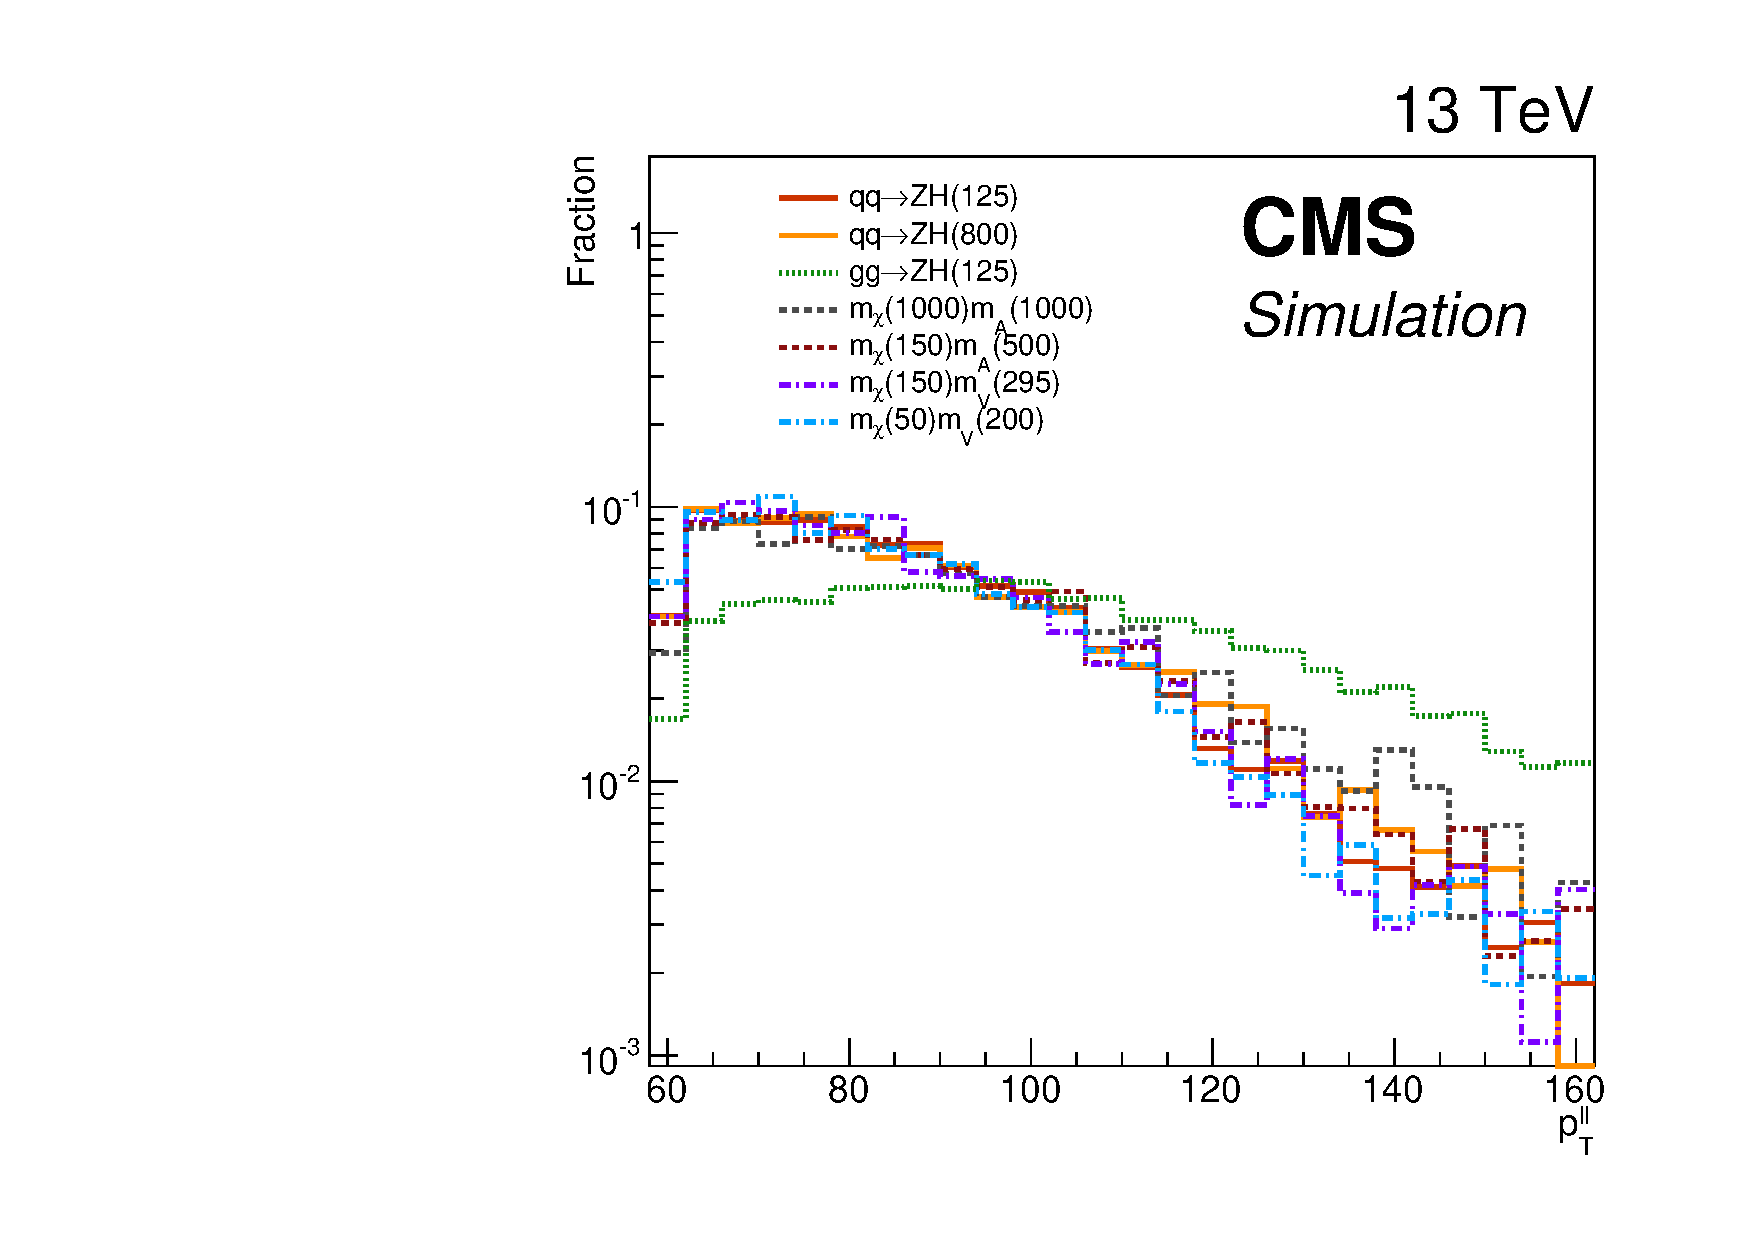
\includegraphics[width=0.42\textwidth]{figures/signals_ptll_presel.pdf}
  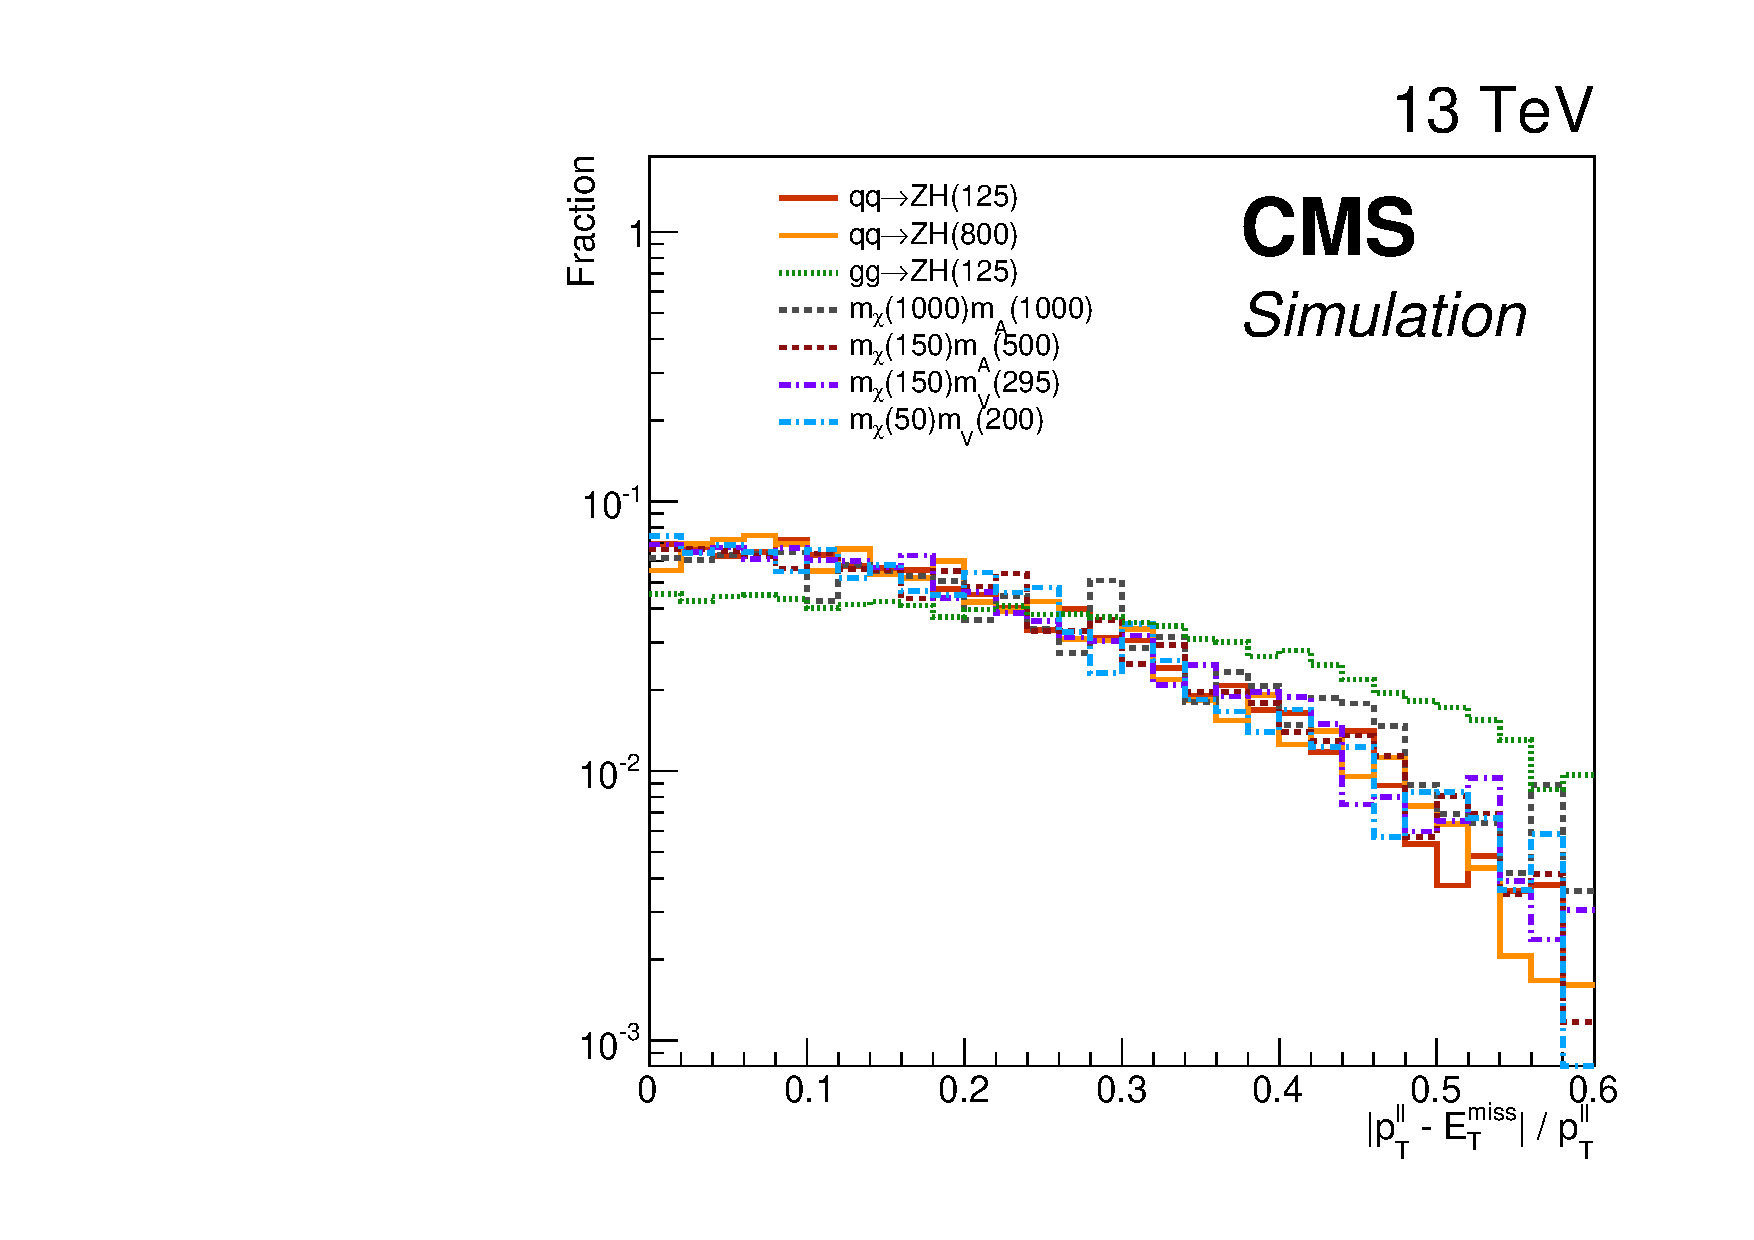
\includegraphics[width=0.42\textwidth]{figures/signals_balance_presel.pdf}
  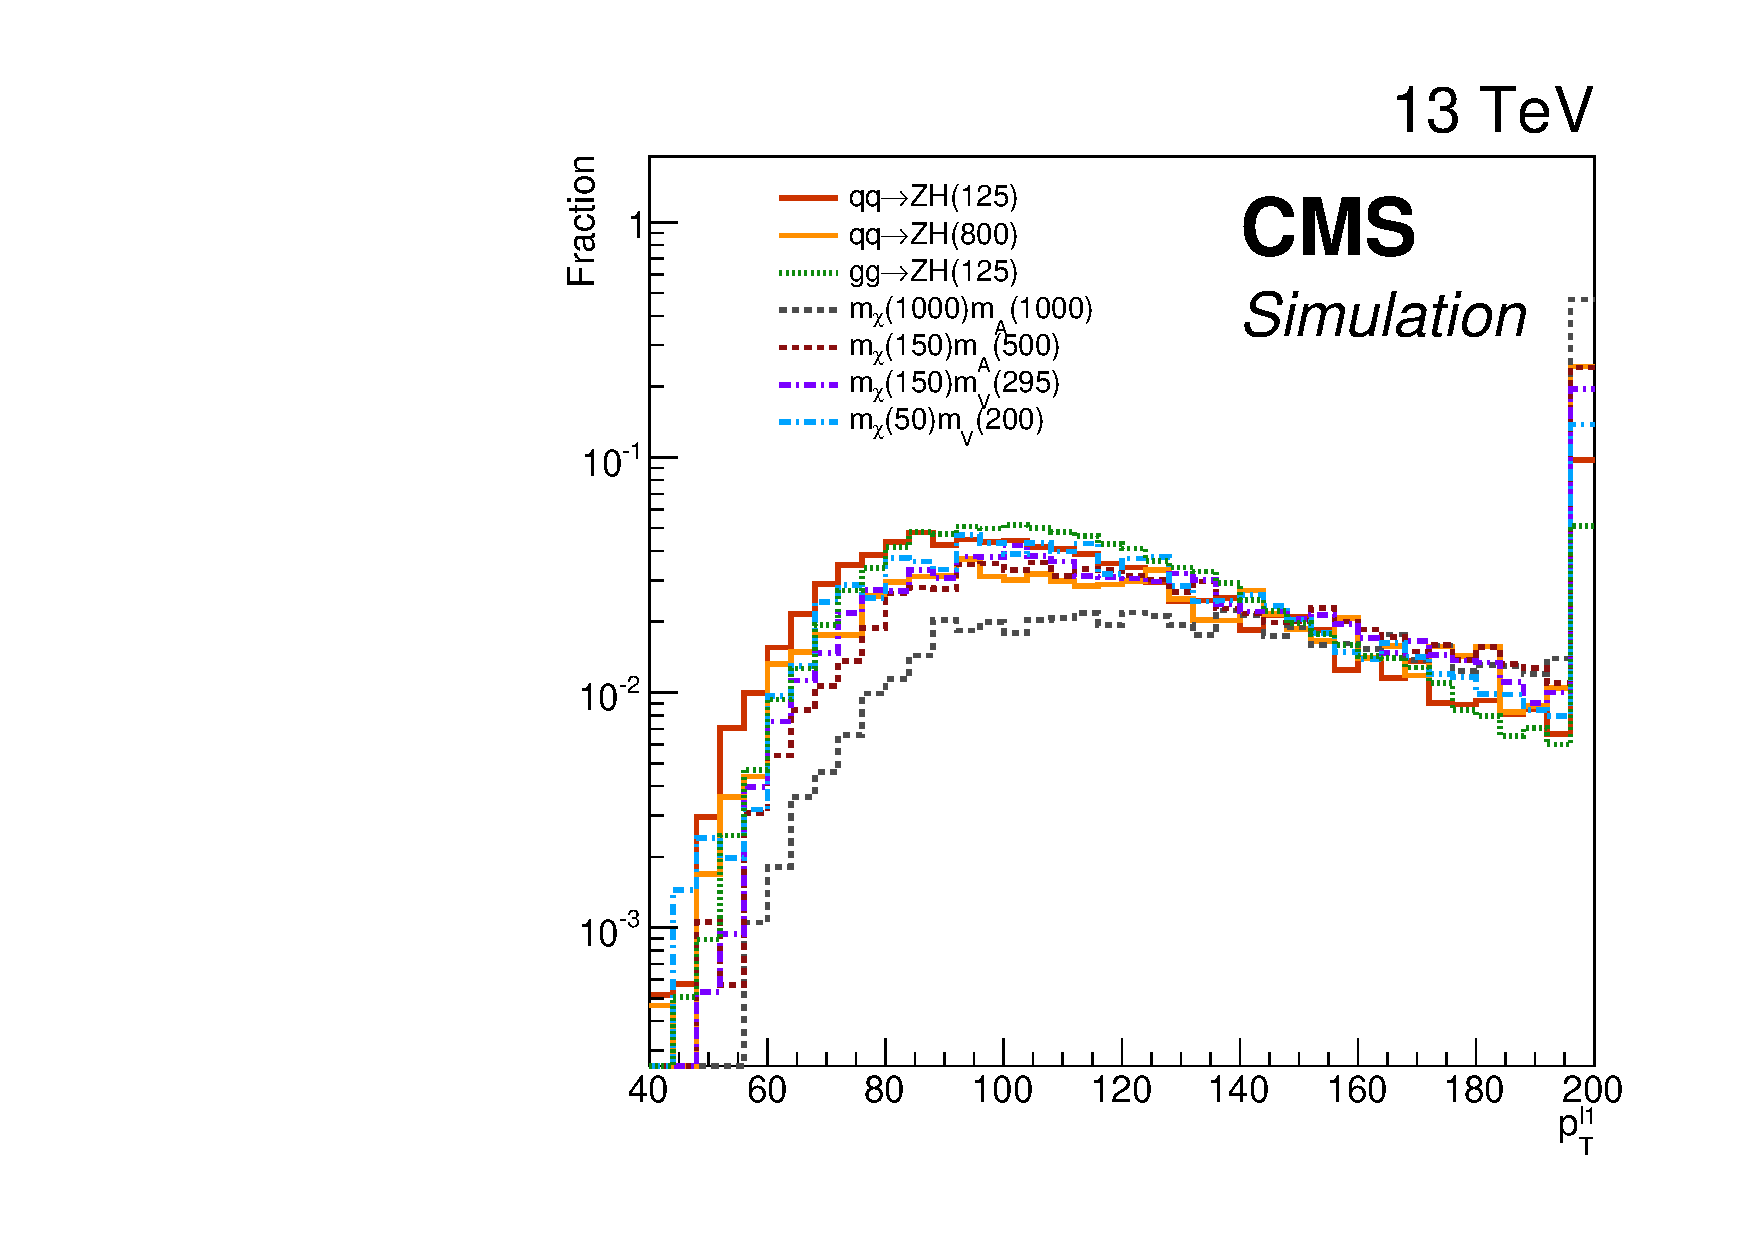
\includegraphics[width=0.42\textwidth]{figures/signals_ptl1_fullsel.pdf}
  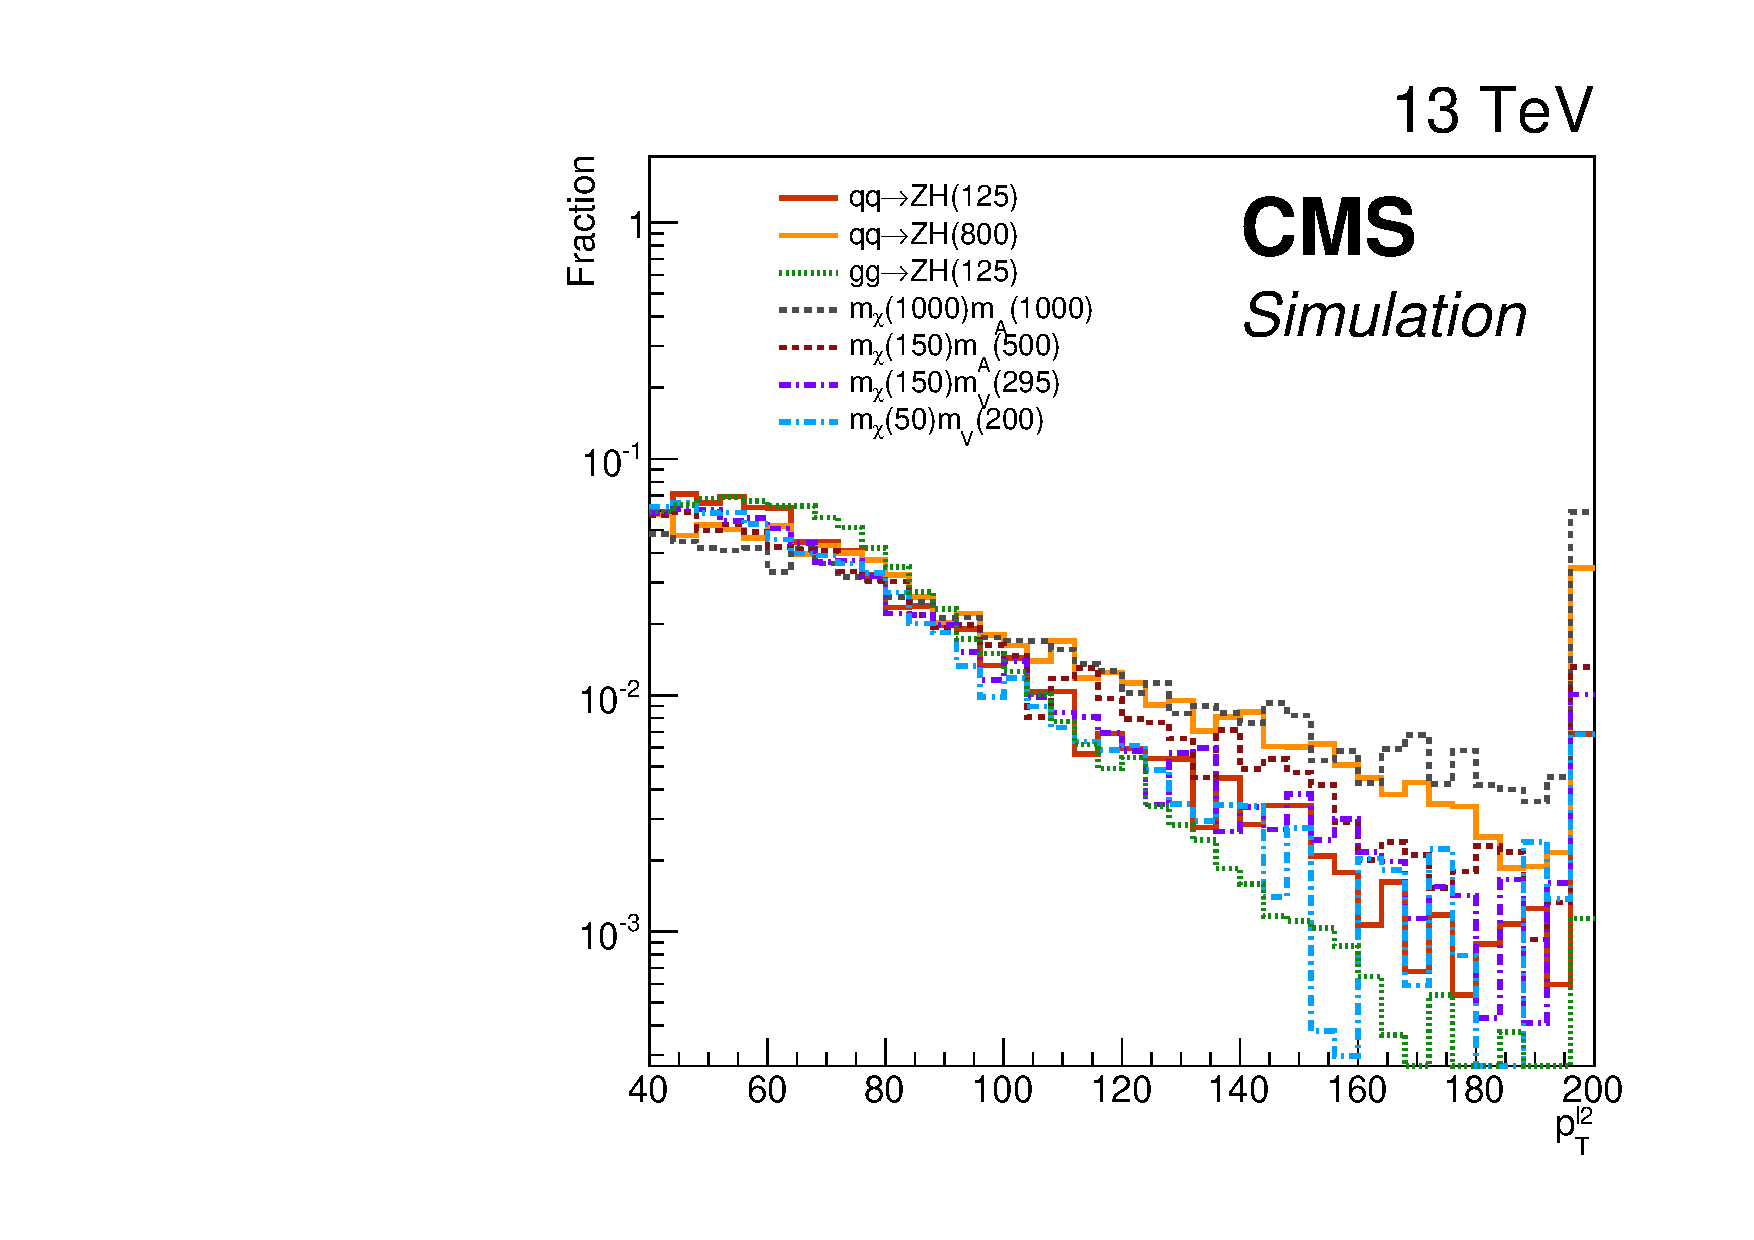
\includegraphics[width=0.42\textwidth]{figures/signals_ptl2_fullsel.pdf}
  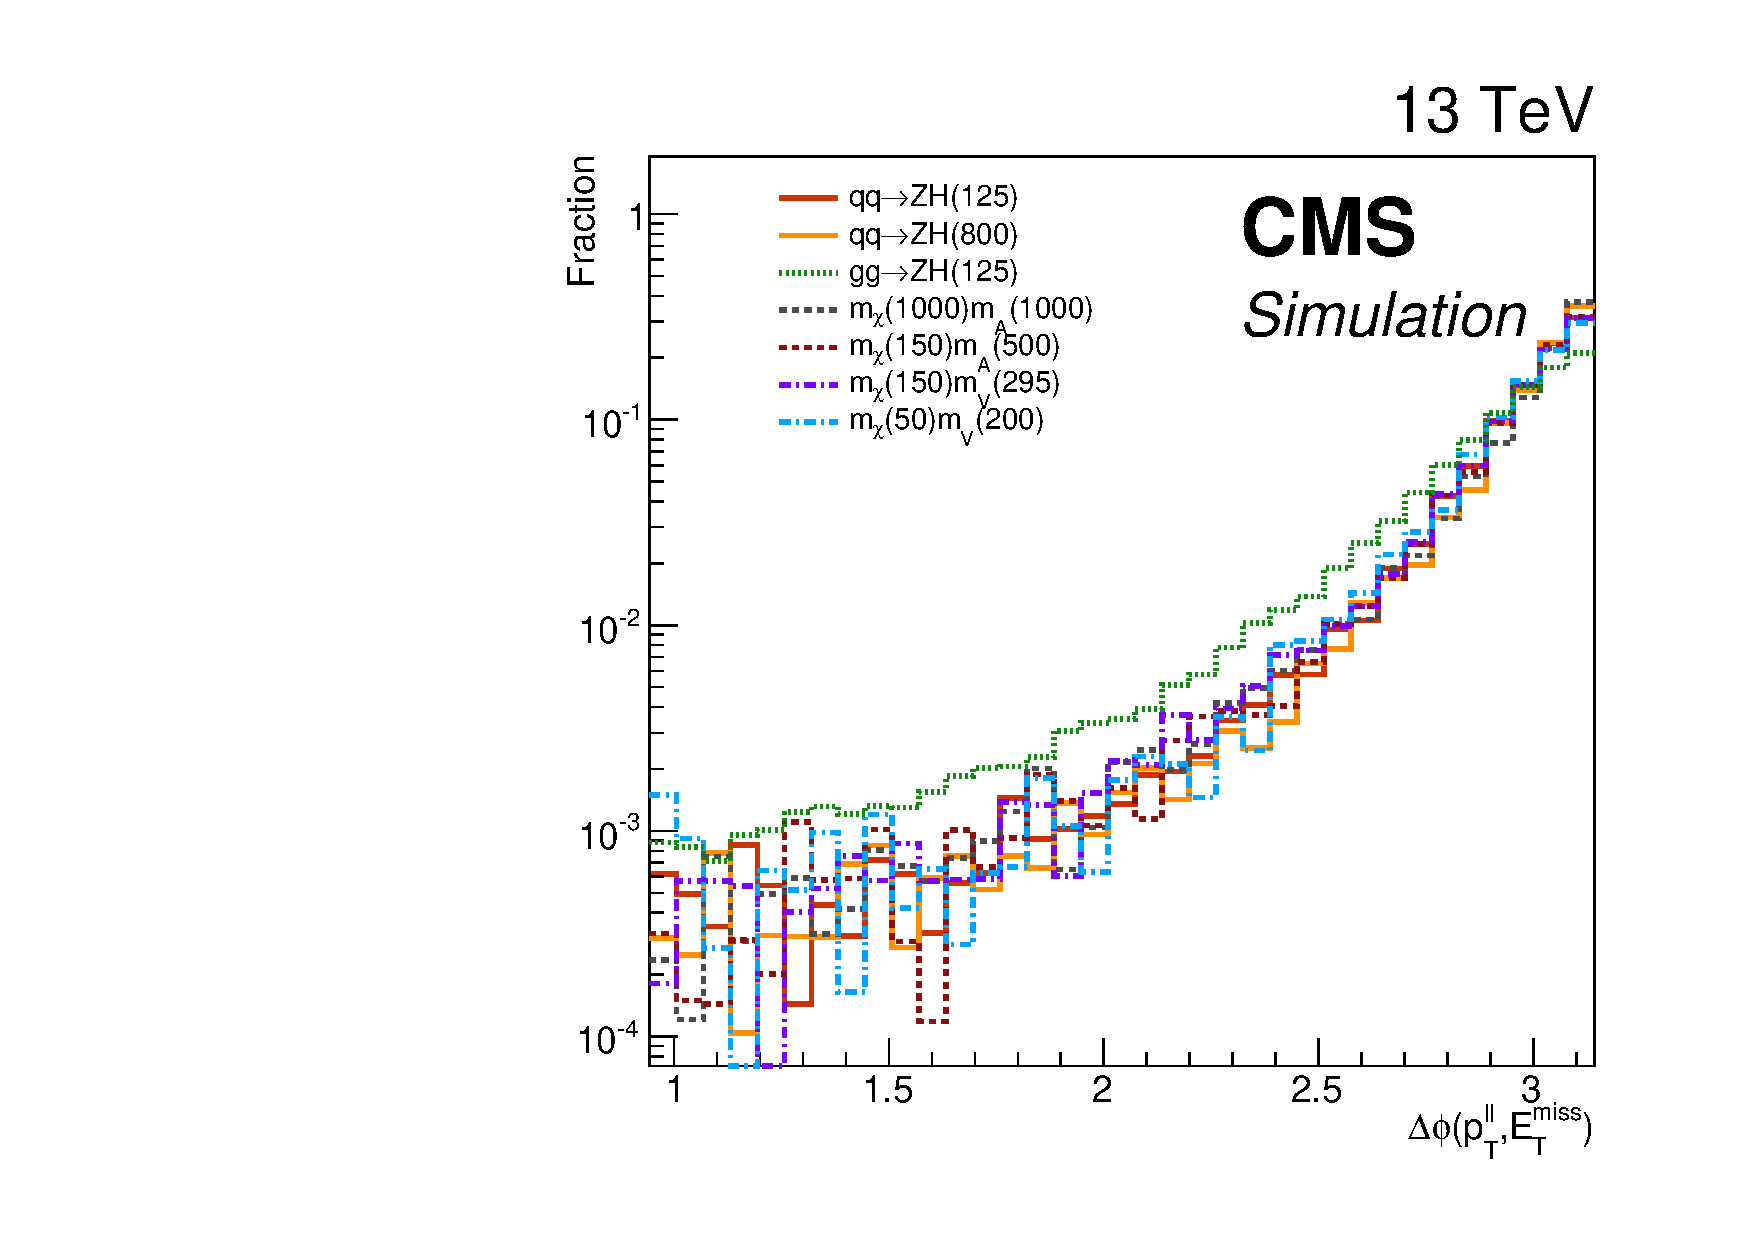
\includegraphics[width=0.42\textwidth]{figures/signals_dphiZMET_nminusone.pdf}
  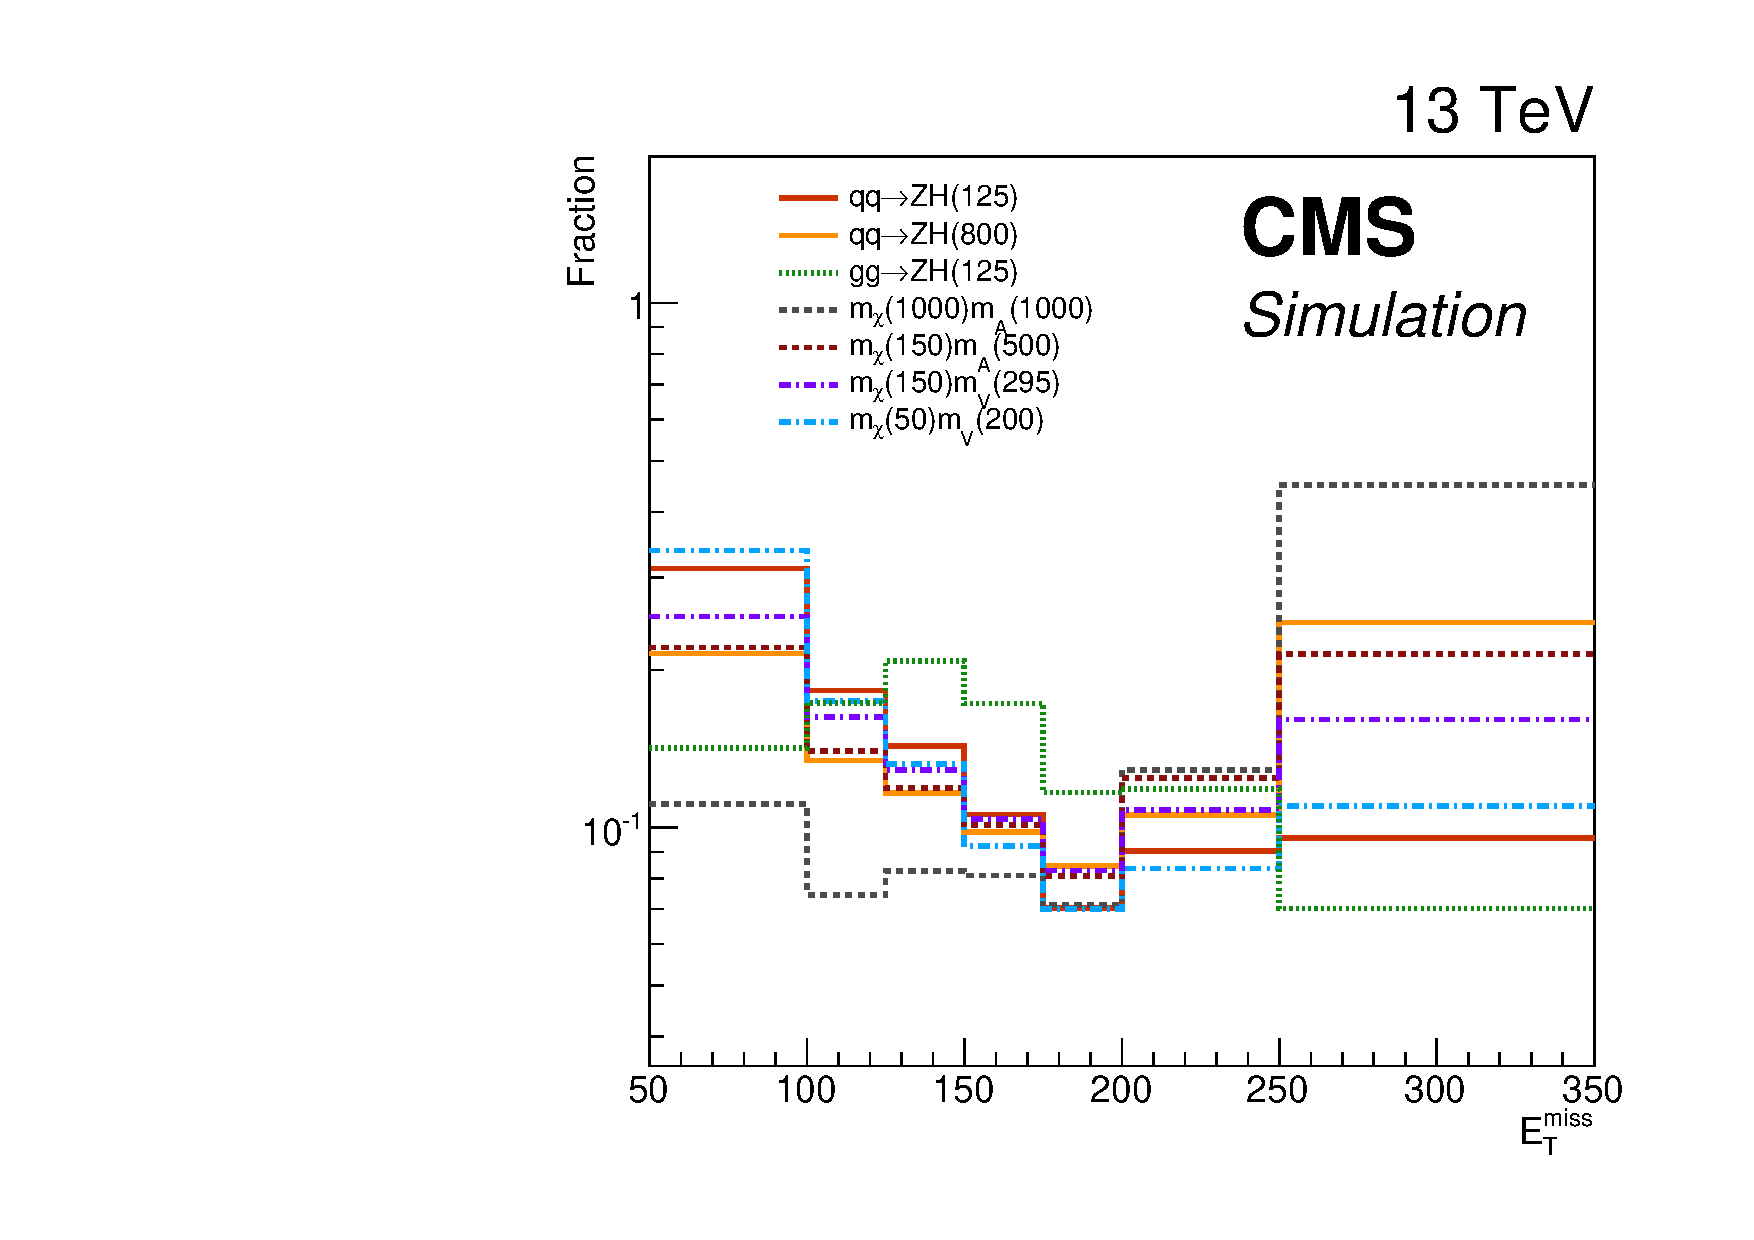
\includegraphics[width=0.42\textwidth]{figures/signals_met.pdf}
  \caption{Comparison of kinematic distributions for a variety of the signal hypotheses. The full distributions are normalized to 1.
  Top left: dilepton $\pt$ (in GeV) in $\zll$ events with $\pt^{\ell\ell} > 60~\GeV$ and $\met > 40~\GeV$. Top right: 
  $|\met-\pt^{\ell\ell}|/\pt^{\ell\ell}$ in $\zll$ events with $\pt^{\ell\ell} > 60~\GeV$ and $\met > 40~\GeV$.
  Center left: leading lepton $\pt$ (in GeV) at final selection level. Center right: subleading lepton $\pt$ (in GeV) at final selection level.
  Bottom left: $\Delta \phi_{\ell\ell-\met}$ at final selection level. Bottom right: the final $\met$ shape used for the shape analysis.}
  \label{fig:signals}
\end{figure}

\begin{figure}[htbp]
  \centering
  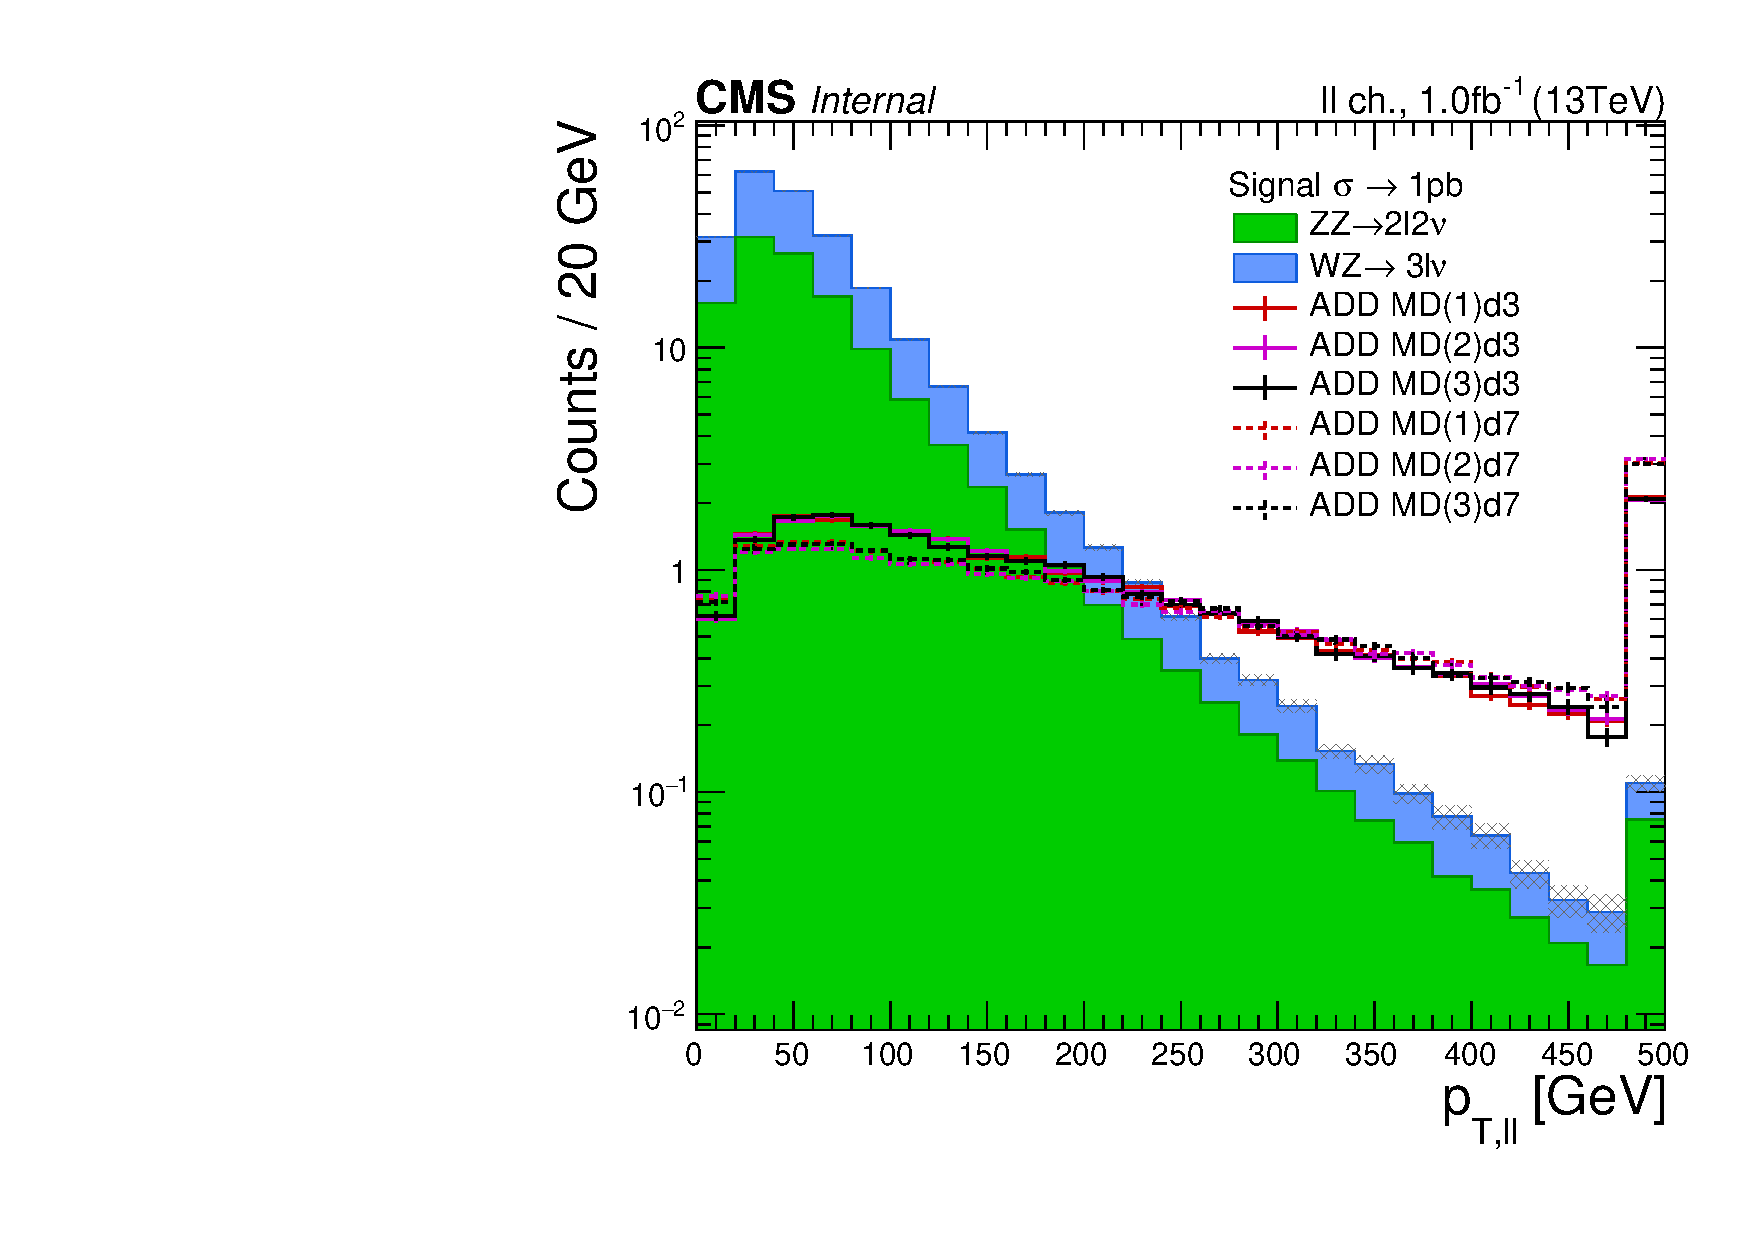
\includegraphics[width=0.48\textwidth]{figures/compare_add.pdf}
  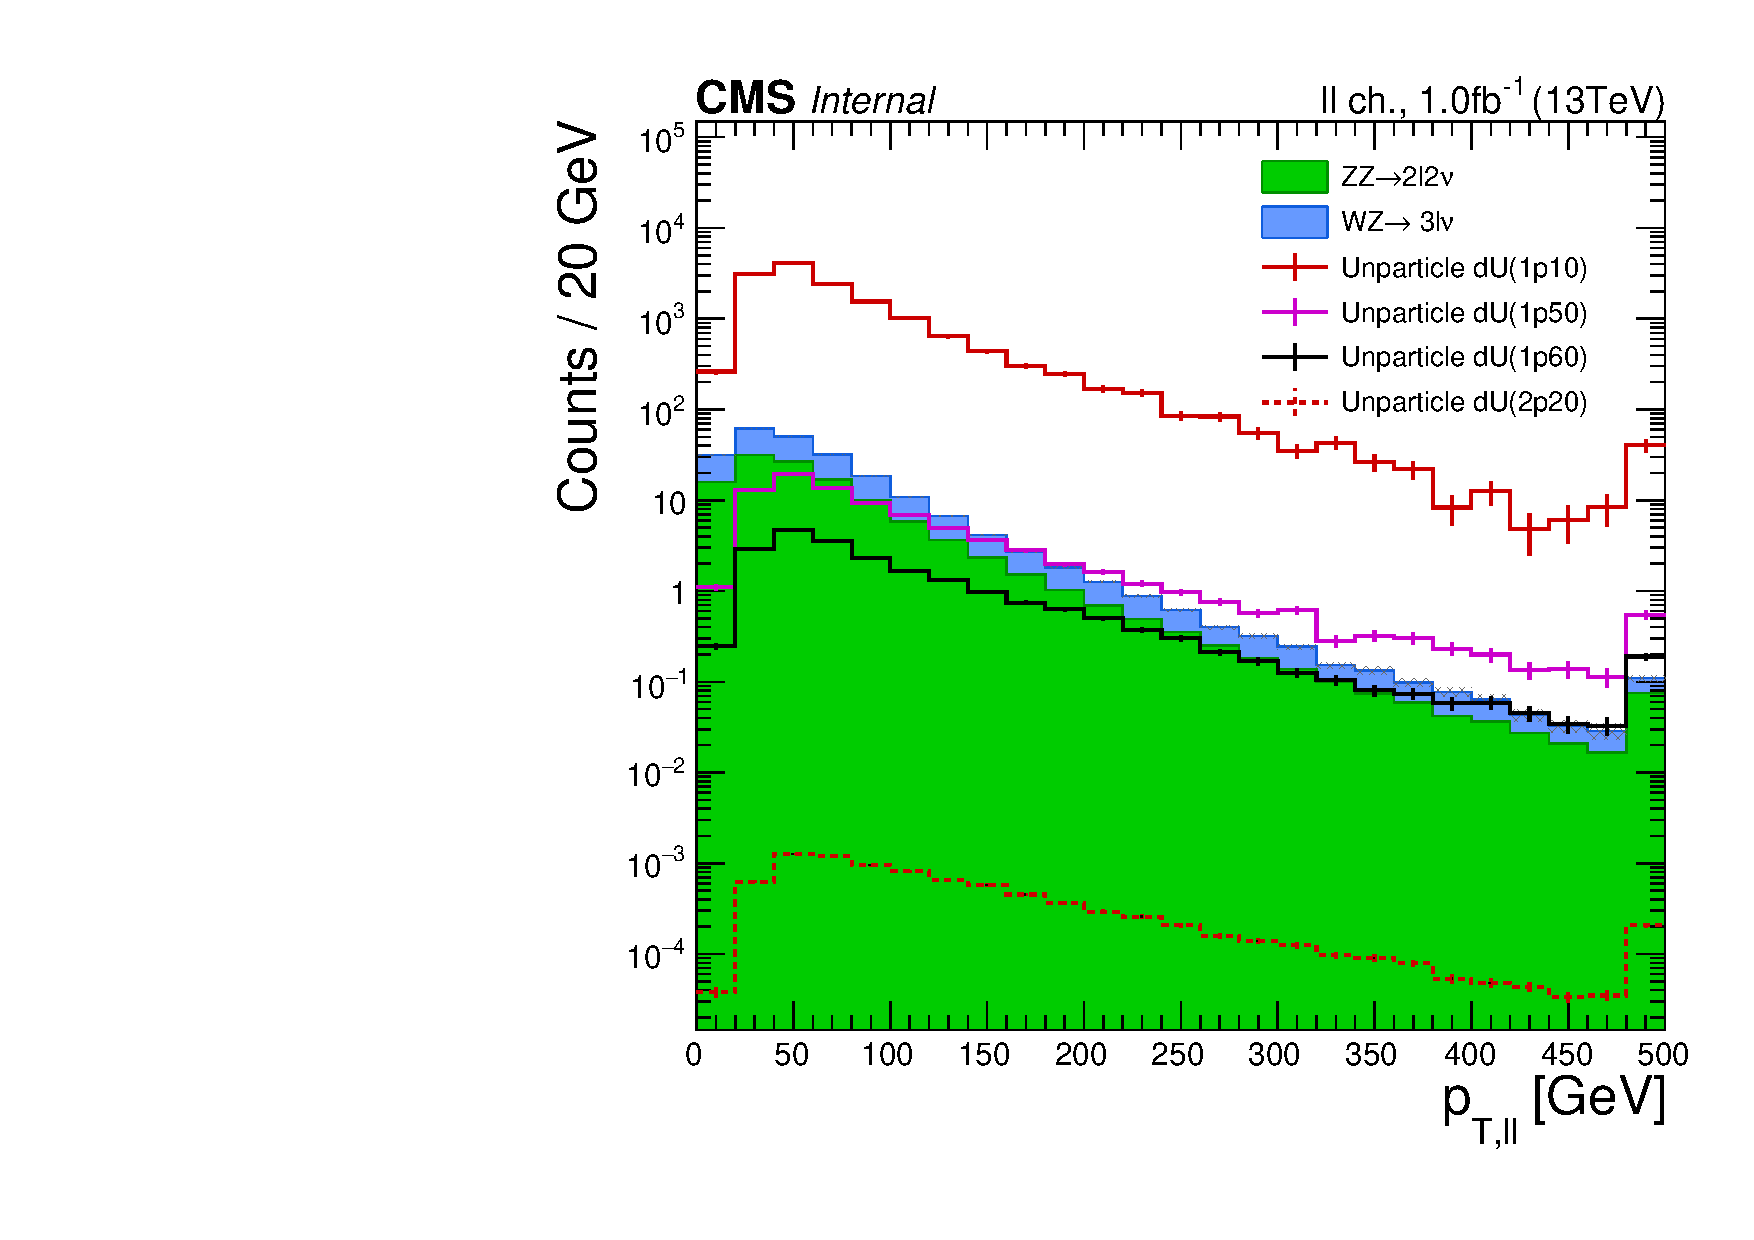
\includegraphics[width=0.48\textwidth]{figures/compare_unparticle.pdf}
  \caption{
    Comparison of reconstructed dilepton transverse momentum ($\pt^{\ell\ell}$) distributions for ADD (left) and unparticle (right) models.
    For the ADD models, cross sections are normalized to $1\pb$.
  }
  \label{fig:moreSignals}
\end{figure}

\section{Triggers}
The triggers used in this work are the so-called ``single and double lepton triggers.''
In general, they are designed to pick out events with one or two electrons or muons,
with momentum of 20 \GeV or more.
The overall trigger efficiency is larger than 99\% and consistent with 1 
after all other selection requirements are applied.

Electron triggers start from Level-1 ECAL primitive objects,
also known as the Level-1 $e/\gamma$ seeds \cite{Khachatryan:2016bia}.
In the ECAL barrel, five strips of five crystals (along the azimuthal direction)
are combined into trigger towers forming a $5\times5$ array of crystals.
The transverse energies detected by the crystals in a single trigger tower are summed
into a trigger primitive by the front-end electronics and sent to off-detector
trigger concentrator cards via optical fibers. 
In the ECAL endcaps, each front-end board computes 5 partial sums of 5 crystals called pseudo-strips,
then sends them to the trigger concentrator card which completes the primitive calculation.
Then, events selected with the Level-1 seed are subject to additional requirements in
the High-Level Trigger including calorimetric isolation requirements.

The Level-1 muon trigger system is informed by all three muon detector subsystems (DTs, CSCs, and RPCs) described in Section~\ref{ss:muonsystem}.
Local track segments are formed within the DTs and CSCs.
Detector hits on the RPCs are used directly for recognition of muon trigger primitive candidates.
The global muon trigger synchronizes and reconciles these pieces of information
from the regional muon primitives to assign momenta, track quality, et cetera to the muon candidates.
Similar to electron primitives, muon primitives passing the L1T also must pass
additional requirements such as isolation in the HLT.

\section{Corrections to the simulated samples}
\subsection{Pileup reweighting}
\label{subsec:puweights}

To match the expected number of pileup interactions in simulation with data,
the reweighting is performed using the minimum bias cross section of 69mb with an uncertainty of 5\%. 
The number of vertices distribution in data and simulation in an inclusive $\Z \to \ell\ell$ sample after the pileup reweighting 
is shown in Figure~\ref{fig:pileup_distribution}.

\begin{figure}[htbp]
  \centering
  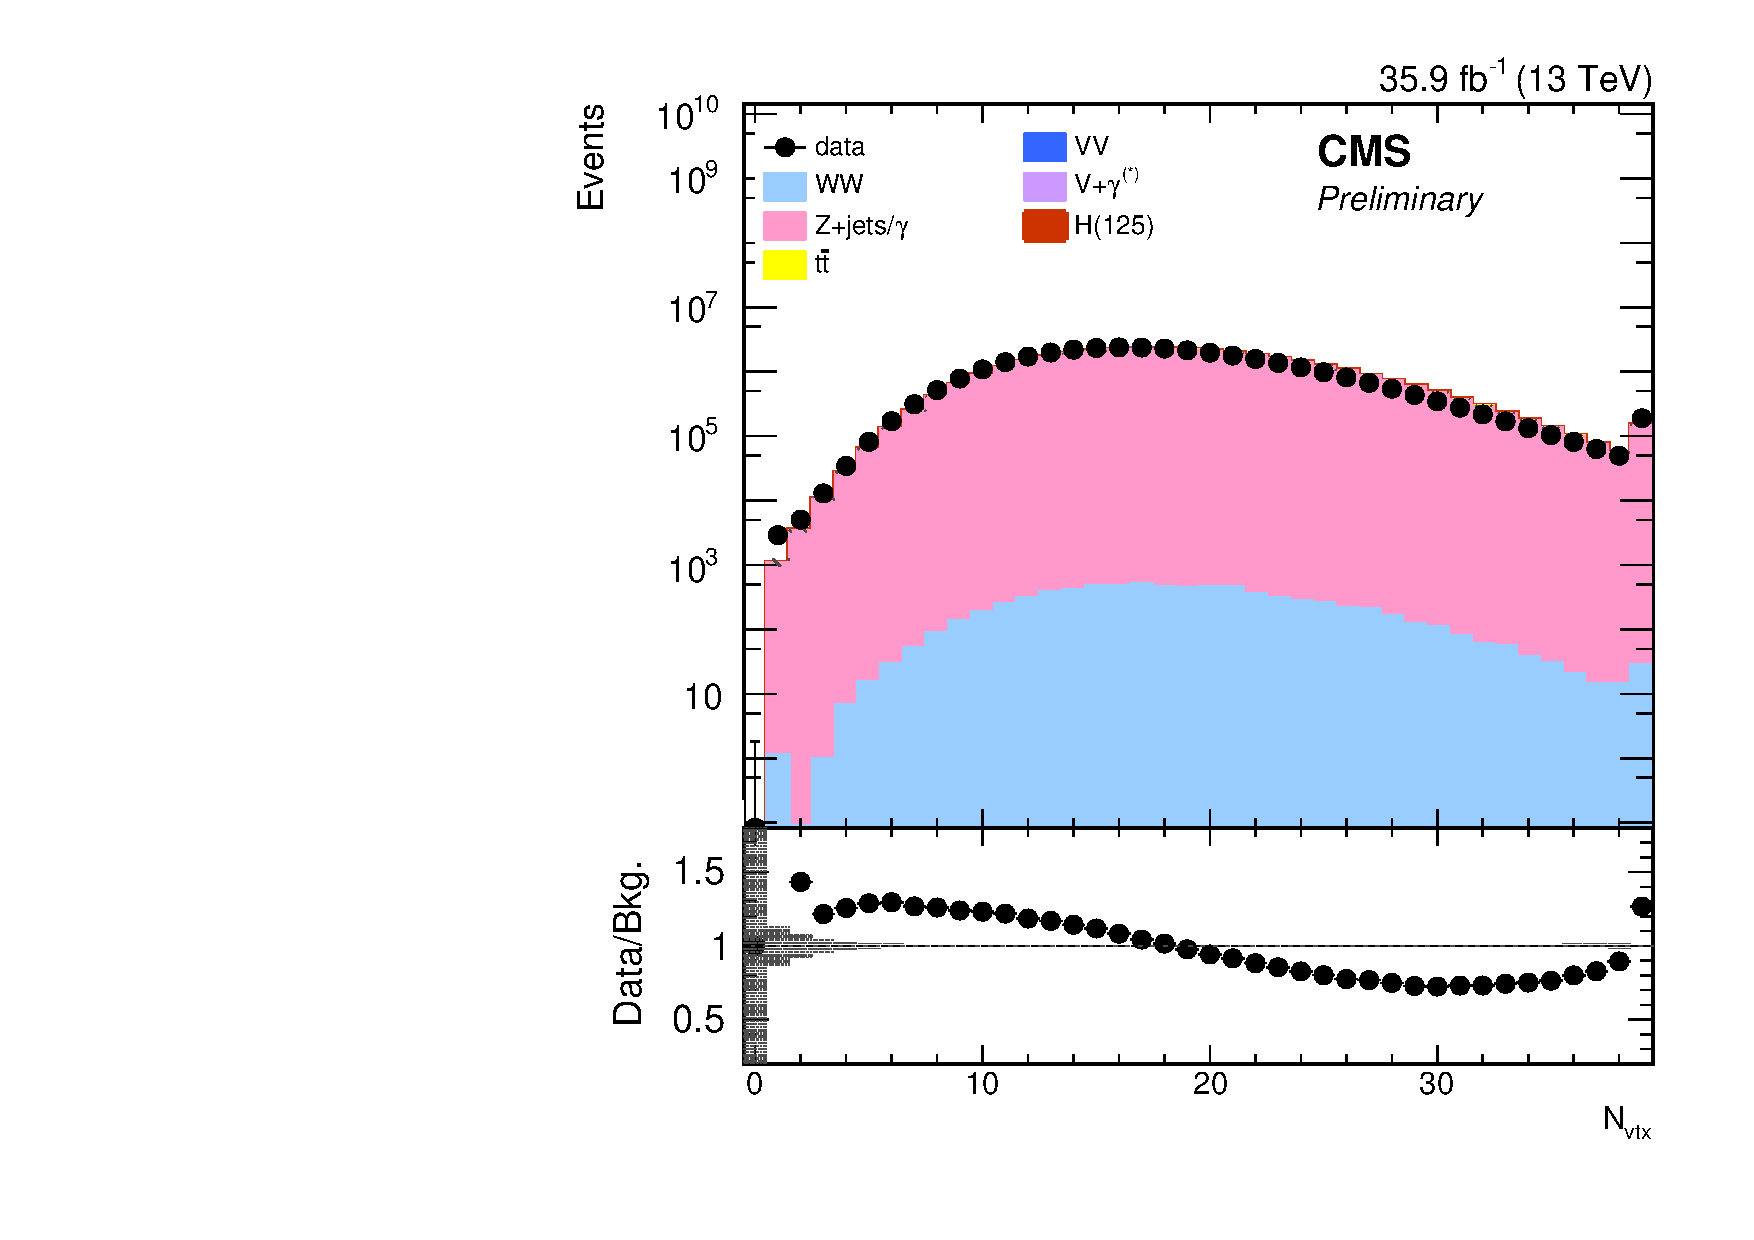
\includegraphics[width=0.48\textwidth]{figures/zll_nvtx_met40_zpt60.pdf}
  \caption{
    Number of reconstructed vertices
    for $\Z \to \ell\ell$ events with $\pt^{\ell\ell} > 60~\GeV$ and $\met > 40~\GeV$.
  }
  \label{fig:pileup_distribution}
\end{figure}

The lepton efficiency studies shown in Chapter~\ref{chap:efficiency} split the data sample in two,
at the point where the HIP effect discussed in Section~\ref{ss:hips} was mitigated.
For these studies, the pileup profile of the relevant simulated samples was reweighted to
the pileup profiles of the two subsets of the data samples, which were substantially different.

\subsection{Trigger efficiencies}
\label{subsec:trigeff}
The efficiency of each of the single and double lepton triggers can be determined 
by measuring the fraction of events which pass the trigger in an unbiased control sample.
Such an unbiased sample may be obtained by using missing transverse energy triggers, as
has been previously done in \cite{Khachatryan:2015oqa}. 
Provided sufficient statistics, the trigger efficiency is parameterized as a function of the 
transverse momentum and pseudorapidity of the lepton or leptons.

The so-called ``trigger soup'' of all of these triggers put together has an efficiency
consistent with 1.
The ratio of trigger efficiency in data versus simulation is also consistent with 1.
For sake of brevity, the exact numbers are omitted.
Any systematic uncertainty from the determination of the trigger efficiency is negligible in
all of the studies presented in this work.

\subsection{Lepton selection efficiencies}
One of the crucial elements in the analysis is the determination of the lepton efficiency scale factors.
Algorithms for selecting good leptons can have different efficiencies in data and simulation.
The ratio of the selection efficiencies in data and simulation constitutes the scale factor.
The scale factors are computed in many bins of electron and muon kinematics to account for relevant dependent effects.
Then, the simulated event weights are multiplied once by the appropriate scale factor for every
lepton identified in that event. A detailed discussion of the methodology to determine these efficiencies is given in Chapter~\ref{chap:efficiency}.

\subsection{Lepton momentum scale and resolution}
\label{subsec:lepres}
The lepton momentum scale and resolution are affected by detector misalignment 
and miscalibration. The calibration procedure includes corrections to both 
data and simulation.
In data momentum corrections are applied differentially in $\pt$, $\eta$, and charge in order to match the value of known resonances. 
These corrections are derived using a multivariate regression technique.
For more details see Ref.~\cite{Chatrchyan:2013dga}. 
In simulation, additional stochastic smearing is applied to match the observed
resolution of the Z boson resonance peak.

For muons, these corrections are known as the Rochester corrections.
The additional effect of uncertainty in the magnetic field is considered.
The methodology and validation is provided in Ref.~\cite{Bodek:2012id}.

\subsection{Higher order corrections}
\label{sec:higher-order-corrections}
The diboson MC samples, including the invisible Higgs signal, are initially generated at electroweak leading-order.

The ZZ and WZ processes are corrected to next-to-leading order in electroweak,
and next-to-next-to-leading order in QCD.
For further details, see Chapter~\ref{chap:dibosons}. 

%In the case of the $\W\Z$ process, a flat correction factor from QCD NLO to NNLO is applied. Its value is 1.109. See reference~\cite{Grazzini:2016swo}.
%Following~\cite{Baglio:113005}, the corresponding NLO EWK correction to WZ production is small, and neglected as a systematic uncertainty.`

For the invisible Higgs boson signal, we apply a differential NLO electroweak correction as a function of the transverse momentum of the $\Z$ boson.
This correction only concerns the Drell-Yan-like $\Z\Hi$ production via $\Pq\Paq$ annihilation
as pictured in the upper left of Figure~\ref{fig:BSMdiagrams}.
The small contributions to the overall $\Z\Hi$ cross section from the gluon-induced, photon-induced, and top-loop production are not corrected in this way.

